\documentclass{article}

\usepackage[utf8]{inputenc}
\usepackage[T1]{fontenc}
\usepackage{lipsum}
\usepackage{graphicx}
\usepackage{amsmath}
\usepackage[margin=1in]{geometry}
\usepackage{titlesec}
\usepackage{enumitem}
\titleformat{\section}
{\LARGE\bfseries}{\thesection}{1em}{}

\titleformat{\subsection}
{\Large\bfseries}{\thesection}{1em}{}

\begin{document}
\pagestyle{empty}

\section*{Diagramma di attività}
\large
\subsection*{Introduzione}
\large
Obiettivi:
\begin{enumerate}
    \renewcommand{\labelenumi}{-}
    \itemsep0em
    \item Riconoscere e acquisire le nozioni per valutare e analizzare diagrammi di attività
\end{enumerate}
Un \textbf{diagramma di attività} è un \textit{diagramma comportamentale} che mostra l'evoluzione di un \textit{flusso di attività}, ognuna delle quali è definita come un'esecuzione non atomica, quindi che può essere interrotta, all'interno di uno \textit{stato}. L'esecuzione di un attività è decomposta in \textit{azioni atomiche}, le quali sono coordinate mediante la ricezione di segnali o di certe informazioni affinchè possano essere avviate. Questa tipologia di modellazione è adoperata per rappresentare il \textit{comportamento} di elementi, quali classi, use case, interfacce, componenti oppure operazioni inerenti a classi.\vspace*{14pt}\\
Si tratta di una variante dei \textit{diagrammi di stato}, in cui ogni \textit{stato} rappresenta l'esecuzione di un'opportuna attività e la transizione da uno stato a quello successivo è generata dal completamento dell'attività stessa. Inoltre, una differenza semantica dei diagrammi di stato è la denominazione posta all'interno dei differenti eventi; infatti si ricorda che in diagrammi di stato i rettangoli figurativi contengono participi, quindi entità che subiscono l'azione o il comportamento, mentre nelle raffigurazioni dei diagrammi di attività è posta la denominazione (\textit{verbo + complemento oggetto}).\vspace{14pt}\\
In UML i diagrammi di attività si basano sulla semantica delle \textit{reti di Petri}, le quali utilizzano termini legati a \textit{transizioni} e a \textit{marcatori di avanzamento}, meglio definiti \textit{token}.\vspace*{14pt}\\
Come avviene per un qualsiasi diagramma, occorre definire quali siano gli strumenti necessari per tale tipologia di modellazione, i quali si differenziano in:
\begin{enumerate}
    \renewcommand{\labelenumi}{-}
    \itemsep0em
    \item Attività
    \item Archi 
    \item Nodi
\end{enumerate}

\subsection*{Attività}
\large
\textit{Definizione informale}\\Un'\textbf{attività} è un comportamento parametrico, rappresentato come un \textit{workflow} coordinato di \textit{azioni}. Il flusso di esecuzione è modellato come un insieme di \textit{nodi} e di \textit{archi}, quest'ultimi permettono di identificare un percorso che renda possibile l'analisi e la lettura del diagramma.\vspace*{14pt}\\
Graficamente un'attività è rappresentata mediante un rettangolo con i vertici smussati, riporta sulla sinistra il nominativo e al suo interno sono posti nodi e archi che compongono il workflow dal punto iniziale a quello finale.\\
\begin{center}
    \includegraphics*[width=0.3\textwidth]{foto 1.png}
\end{center}

\subsection*{Azione}
\large
\textit{Definizione informale}\\Un'\textbf{azione} è un elemento che indica un singolo passaggio \textit{atomico}, quindi a differenza di una attività non potrà essere interrotto.\vspace*{14pt}\\
Sono rappresentate graficamente mediante rettangoli con i vertici smussati, dove al loro interno sono posto i nomi dell'azioni.\\
\begin{center}
    \includegraphics*[width=0.3\textwidth]{foto 2.png}
\end{center}
Come da immagine, un'azione può avere sia archi in entrata che archi in uscita, specificandone la direzione dei propri flussi di dati. Aggiungendo, un'azione non potrà essere avviata affinchè le sue \textit{condizioni di input} non saranno soddisfatte.\vspace*{14pt}\\
Al di sopra e al di sotto di ogni azione, possono essere specificate delle \textit{pre-condizioni} e delle \textit{post-condizioni}, le quali hanno valenza soltanto nel punto di workflow specificato, quindi prima dell'esecuzione e al completamento dell'esecuzione.\vspace*{14pt}\\
Alcune azioni specifiche indicano degli eventi, e vengono rappresentate graficamente in maniera differente:
\begin{enumerate}
    \renewcommand{\labelenumi}{-}
    \itemsep0em
    \item Inviare un messaggio
    \item Accettare un messaggio
    \item Tempo ripetuto 
\end{enumerate}
\begin{itemize}[label={ }]
    \renewcommand{\labelenumi}{-}
    \item 
    \begin{tabular}{c c c}
        \begin{minipage}[b]{0.3\textwidth}
            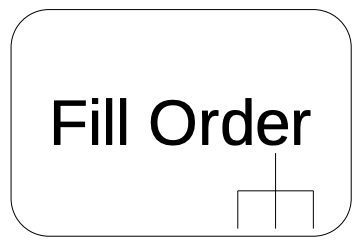
\includegraphics[width=\textwidth]{foto 3.png}
        \end{minipage}
        &
        \begin{minipage}[b]{0.3\textwidth}
            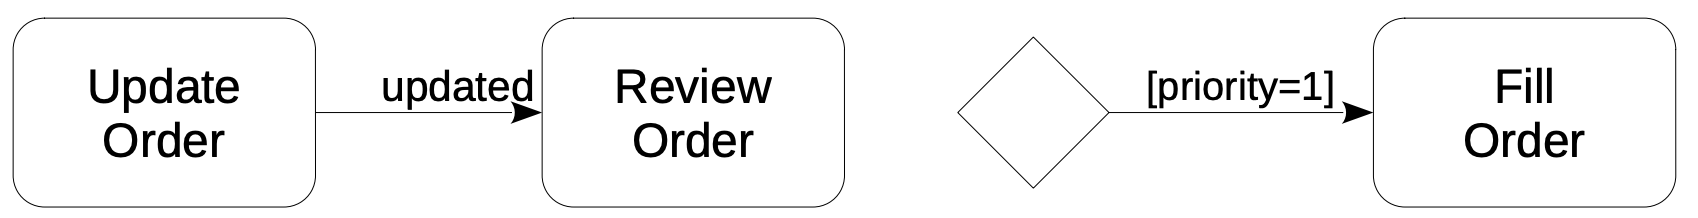
\includegraphics[width=\textwidth]{foto 4.png}
        \end{minipage}
        &
        \begin{minipage}[b]{0.3\textwidth}
            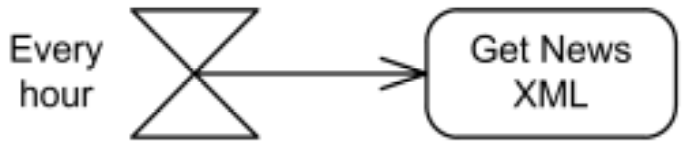
\includegraphics[width=\textwidth]{foto 5.png}
        \end{minipage}
    \end{tabular}
\end{itemize}

\subsection*{Chiamata comportamentale}
\large
\textit{Definizione informale}\\Una \textbf{chiamata comportamentale} rappresenta un collegamento ad un'altra attività, indicando un livello informativo per una certa azione molto più dettagliato.\vspace*{14pt}\\
Graficamente è riportato un simbolo all'interno del rettangolo dell'azione, che ne specifica un ulteriore diagramma di attività, univoco per quell'atto.\\
\begin{center}
    \includegraphics*[width=0.2\textwidth]{foto 6.png}
\end{center}

\subsection*{Archi}
\large
\textit{Definizione informale}\\Un \textbf{arco} è una connessione diretta tra due azioni, lungo i quali possono scorrere i \textit{marcatori di attività} dall'origine fino alla destinazione. Spesso è descritta come una generalizzazione del flusso di controllo e degli archi del flusso degli oggetti.\\
=======
\textit{Descrizione informale}\\Un \textbf{arco} è una connessione diretta tra due azioni, lungo i quali possono scorrere i \textit{marcatori di attività} dall'origine fino alla destinazione. Spesso è descritta come una generalizzazione del flusso di controllo e degli archi del flusso degli oggetti.\\
>>>>>>> 6ebde9cf38f3c79aea2376a7c27143d6c51f4541
=======
\textit{Descrizione informale}\\Un \textbf{arco} è una connessione diretta tra due azioni, lungo i quali possono scorrere i \textit{marcatori di attività} dall'origine fino alla destinazione. Spesso è descritta come una generalizzazione del flusso di controllo e degli archi del flusso degli oggetti.\\
>>>>>>> 6ebde9cf38f3c79aea2376a7c27143d6c51f4541
\begin{center}
    \includegraphics*[width=0.7\textwidth]{foto 7.png}
\end{center}
Sono rappresentati graficamente come una freccia direzionata, dove al di sopra è posta la figura della \textit{guardia}; il compito della guardia consiste nel valutare se i marcatori possano attraversare l'arco. A differenza delle condizioni di un'azione, una guardia è valutata durante il \textit{runtime} dei token, per cui possono arrestare il loro flusso nel momento esatto in cui sono ritratti nel passaggio di un evento ad uno successivo.

\subsection*{Connettore}
\textit{Definizione informale}\\Un \textbf{connettore} indica un termine tecnico adoperato per una migliore e agevole lettura del diagramma di attività.\vspace*{14pt}\\
Infatti l'obiettivo ricade nel posizionamento di certe connessioni in modo che non siano di intralcio durante la lettura del \textit{workflow} di \textit{token}. Un esempio figurativo può essere:\\
\begin{center}
    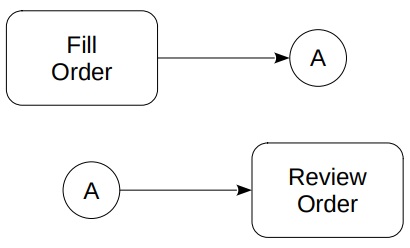
\includegraphics[width=0.32\textwidth]{foto 8.png}
\end{center}

\subsection*{Lettura del diagramma di attività}
\large
\begin{center}
    \includegraphics*[width=1\textwidth]{foto 9.png}
\end{center}
L'attività rappresentativa è denominata \textit{Process Order}, in cui al suo interno sono presenti le \textbf{swimline}. Una \textit{swimline} è un raggruppamento di attività eseguite da una stessa entità, per cui nell'esempio proposto, indicano flussi elaborati parallelamente.\vspace*{14pt}\\
L'inizio del flusso generalmente è indicato con un \textbf{pallino nero} posto in alto a sinistra da cui inizieranno a defluire i differenti token. Scorrendo gli elementi interni, si nota la presenza di un rettangolo con vertici non smussati; si tratta di un \textbf{oggetto}, ossia un'istanza che descrive uno stato aggiuntivo di un'azione, come avviene tra \textit{Receive Order} e \textit{Requested Order}, in cui il secondo citato è oggetto dell'azione o nodo attività \textit{Receive Order}. Per cui indica un livello informativo più dettagliato in cui un ordine può essere ricevuto se non prima sia stato richiesto quel determinato ordine.\vspace*{14pt}\\
I \textit{rombi} descrivono \textbf{punti decisionali}, che permettono di interpretare differenti flussi a seconda delle informazioni processate e valutate, come può essere il conseguimento elaborativo dell'ordine oppure nell'eliminazione dello stesso qualora sia rigettato.\vspace*{14pt}\\
Analizzate le \textit{swimline} precedentemente, le quali permettono l'avvio di \textit{workflow} paralleli, la destinazione è rappresentata graficamente mediante un \textbf{pallino nero} inciso all'interno di una circoferenza.

\subsection*{Notazioni aggiuntive}
\large
Di seguito sono riportate notazioni utilizzate per facilitare la lettura di diagrammi simili, aggiungendo inoltre strumenti in grado di rendere maggiormente espressiva tale modellazione.\vspace*{14pt}
\textit{Definizione Partizione di attività}\\Una \textbf{partizione di attività} raggruppa un insieme di azioni che hanno caratteristiche comuni.\vspace*{14pt}\\
Le partizioni garantiscono una visualizzazione dei comportamenti invocati da parte delle stesse azioni, e spesso corrispondono figurativamente a unità orizzontali, le quali pongono una suddivisione in \textit{layer} durante la lettura del diagramma. Concludendo, solitamente per ogni \textit{layer} è descritto un nominativo che corrisponda ad elementi organizzativi, attori oppure ad ulteriori modelli.\\
\begin{center}
    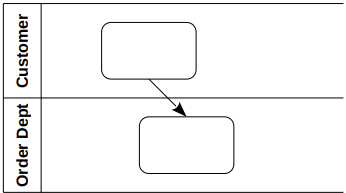
\includegraphics[width=0.4\textwidth]{foto 10.png}
\end{center} 
Come da esempio, una partizione di attività è data dall'\textit{attore} Customer e dall'\textit{elemento organizzativo} Order Dept.\vspace*{14pt}\\
\textit{Definizione Sezione interrompibile}\\Una \textbf{sezione interrompibile} è una tipologia di insieme di attività, il quale provvede ad un meccanismo per la distruzione di tutti i \textit{marcatori} e l'eliminazione di tutti i \textit{comportamenti} posti all'interno della regione dedicata. \vspace*{14pt}\\
Quando un \textit{marcatore} attraversa un \textit{arco predefinito} detto \textbf{interrupting edge}, spesso rappresentato come una \textit{lightning bolt}, tutti i \textit{token} sono distrutti e i comportamenti immessi nella sezione sono terminati.

\subsection*{Lettura sezione interrompibile}
\large
\begin{center}
    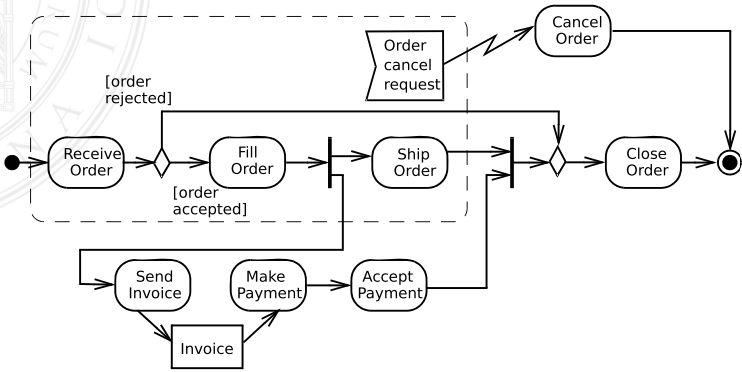
\includegraphics[width=0.85\textwidth]{foto 11.png}
\end{center}
L'esempio raffigura nuovamente il processo di elaborazione di qualsiasi tipologia di ordine. Sono posti stessi elementi descritti prima, ma con alcune differenze.\vspace*{14pt}\\
L'area trateggiata identifica la \textbf{sezione interrompibile}, quindi pone il meccanismo specializzato per l'interruzione di ogni \textit{workflow} qualora si verifichino certe condizioni. Ciò avviene in casistiche in cui l'ordine effettuato dovesse essere cancellato, provocando l'eliminazione di ogni possibile token e terminando tutti i \textit{behaviors}. Graficamente è rappresentato mediante una certa tipologia di \textit{azione}, ossia l'\textit{accettazione del messaggio}, collegato tramite una \textit{lightning bolt} ad un'azione al di fuori della regione, che provvederà al raggiungimento del nodo di destinazione.\vspace*{14pt}\\
Contrariamente i \textit{marcatori} possono proseguire per flow alternativi, comprendenti l'esecuzione dell'ordine oppure il rigetto dello stesso.
\end{document}